\chapter{Compression on the basis of equivalence classes}

\section{Related Compression Techniques}
Compression of sequencing short reads becomes crucial with the lowering cost of sequencing technology. The rapid technological development enables the generation of petabytes of data on servers worldwide. Apart from size, often succinct representation \citep{Pritt2016} also yields almost accurate results with a much smaller memory footprint. Nucleotide sequence compression can largely be divided into two paradigms, one is reference based compression where the reference is needed to transfer to the decoder end along with the compressed data ~\citep{Canovas2014}, \citep{Fritz2011}, \citep{Li2014}. Another is reference free compression, \citep{adjeroh2002dna},\citep{Bonfield_2014}, \citep{Hach2012} where the read sequences are compressed independent of reference sequence, barring the burden of transferring reference. Such compressions are commonly known as \Denovo compression. A robust and widely used \denovo compressor, LEON \citep{Benoit2015}, constructs a de Bruijn graph from the k-mer counts table extracted build on the reads. Reads are then mapped to the newly constructed de Bruijn graph, and are stored in form of anchor address, read size and bifurcation list.   

Reference based compressions start with the BAM file produced by state of the art aligners such as \Bowtie. Typically these algorithms store the edits after aligning the sequences to reference. \citet{Fritz2011} is one such widely used tool A serious bottleneck of such approaches is to store all meta information in the BAM file which can be regenerated re-aligning the reads to the provided reference sequence. This problem is partially addressed by fastq \citep{bonfield2013compression}, where a new alignment technique is being implemented to navigate through the problem of storing meta-data footprint. 



There are few mappers which does compression of genome/transcriptome for the better mapping, and also compress reads on the way. Recently published CORA ~\citep{Yorukoglu2016} is a compressive read mapper. The working principle of CORA is interesting and worth mentioning as concept of equivalence classes is also used there, but carries a different meaning. CORA converts the fastq reads to non redundent k-mer sets. Furthermore, CORA does a redundancy removal on reference genome, by self mapping. The positions where a k-mer maps form an equivalence class. Two equivalence classes are regarded as concordant if all positions of one equivalence class are in one nucleotide shift distance from another equivalence class. 

Apart from reference based and \denovo mappers, few mappers lie in the middle, which  stores a part of the reference that is shared between reads. Kpath \citep{Kingsford2015} is a tool that stores the shared reference as that acts as a backbone for a statistical generative model. An arithmetic coding is performed on the reads.

\begin{figure}[!ht]
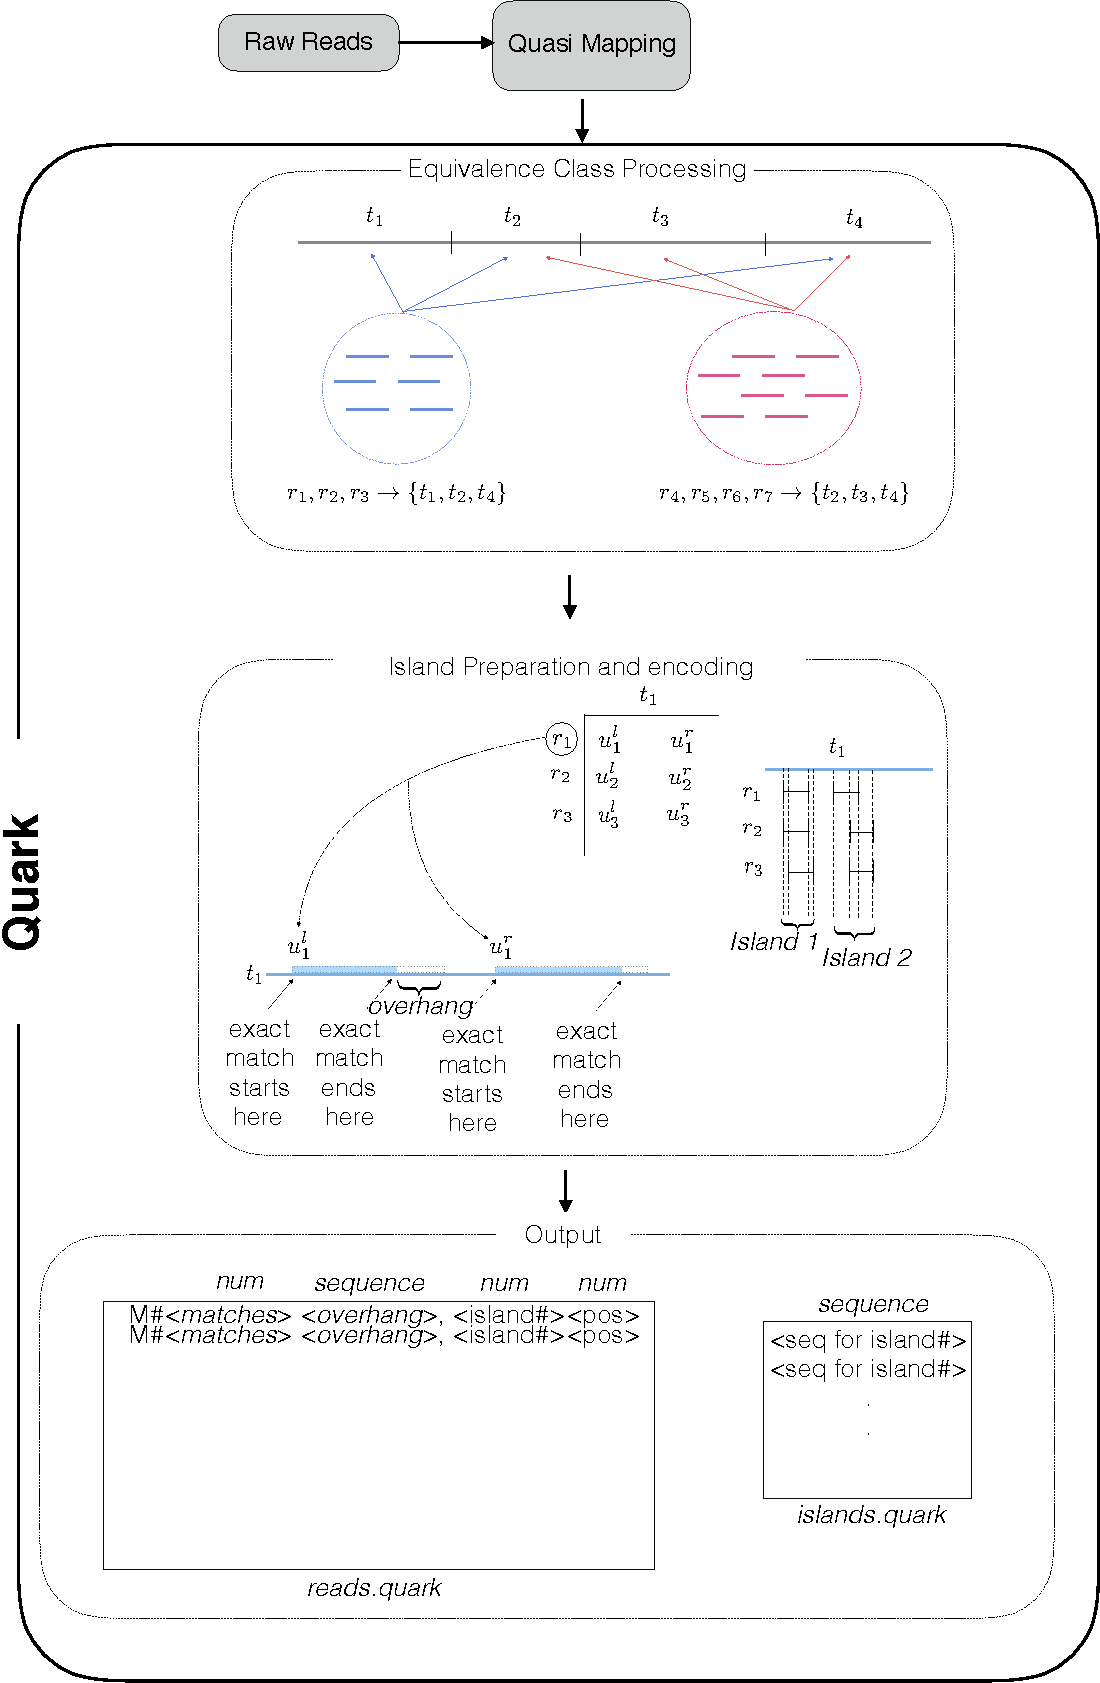
\includegraphics[width=\textwidth]{Figures/quark_overview4-crop}
\centering
\caption{\label{fig:overview}An overview of the \quark pipeline. Equivalence classes are computed using \qm, Reads within classes along with the positions are then used find out the exact match length and the overhang portion. Islands are simultaneously processed from the intervals. In the last steps encoded reads along with the islands are stored as \quark output.}
\end{figure}

